\section[Depth Sensor]{Testing driftnode}

\subsection[Overview]{Commercially available depth transducer}

\begin{figure}[h]
	\begin{center}
	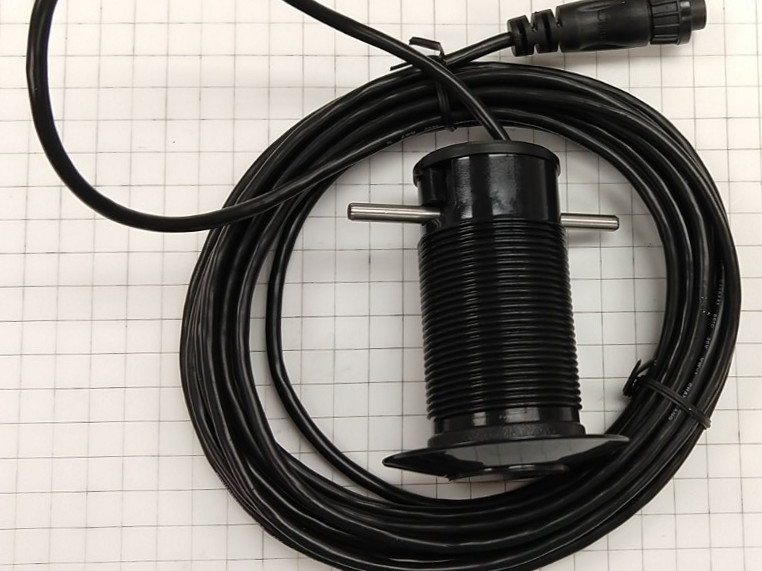
\includegraphics[width=0.4\columnwidth]{driftnode/garmin.jpg}
	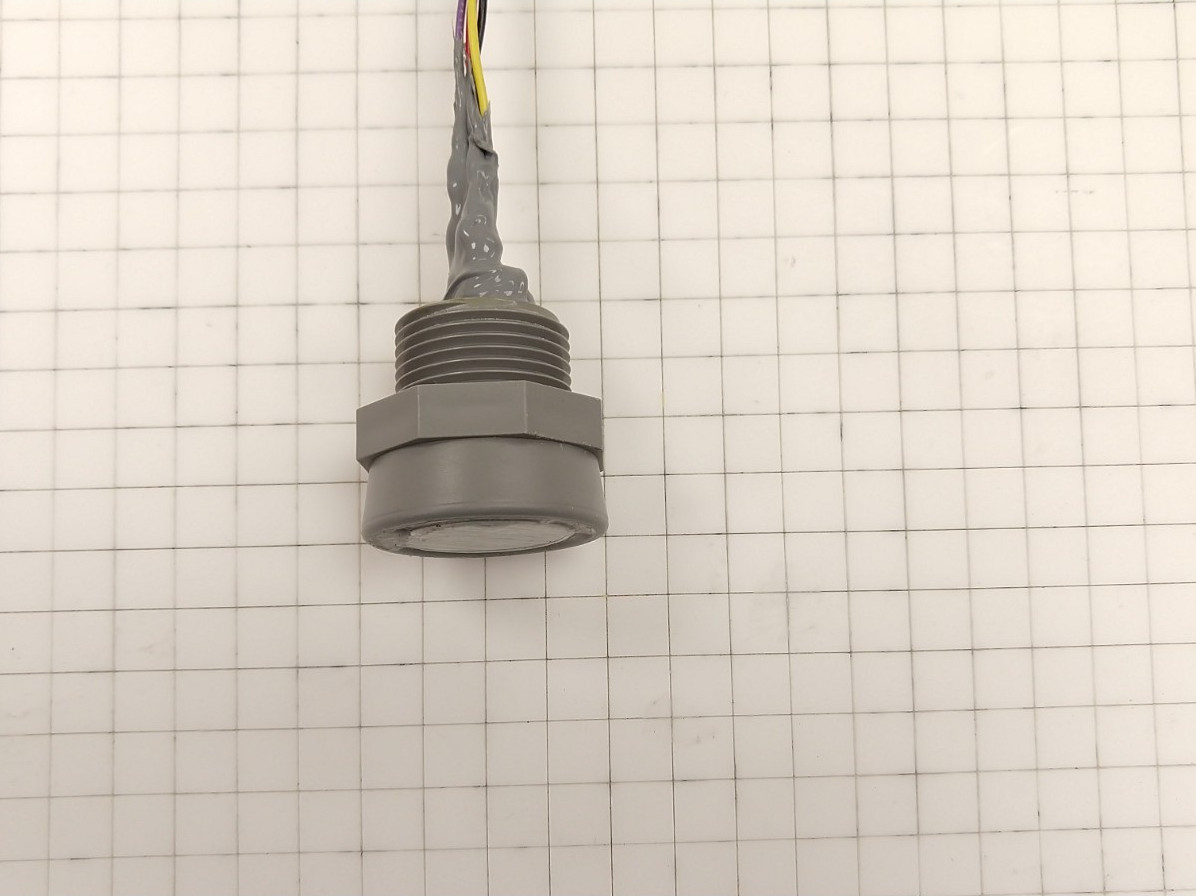
\includegraphics[width=0.4\columnwidth]{driftnode/maxbotix.jpg}
	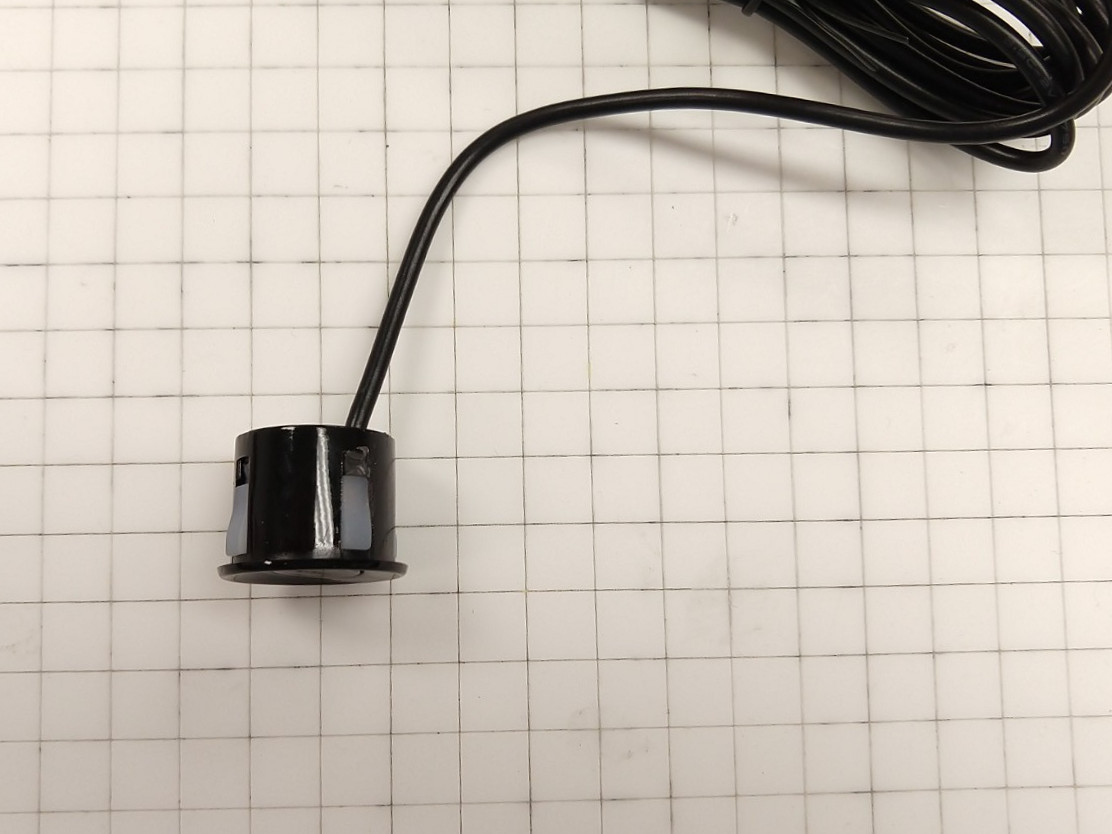
\includegraphics[width=0.4\columnwidth]{driftnode/jsnsr04t.jpg}
	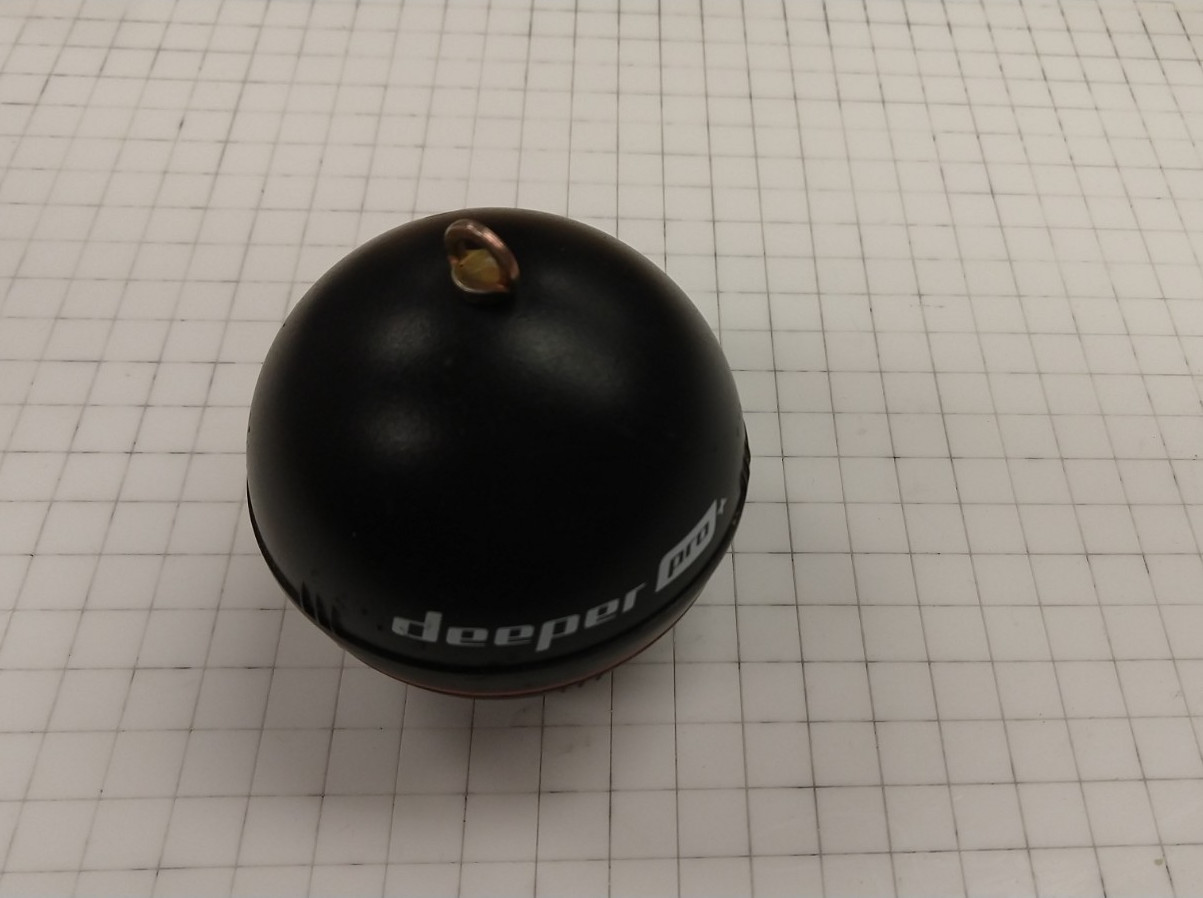
\includegraphics[width=0.4\columnwidth]{driftnode/fishfinder.jpg}
	\caption[Various range finder]{
		(Top Left) Garmin GDT 43 uses NMEA 2000 
		(Top Right) MaxBotix MB7380 use analog voltage output 
		(Bottom Left) JSN-SR04T use trigger and echo timing
		(Bottom Right) Deeper Smart Sonar PRO proprietary fish finder 
	} \label{fig:sonarsensors}
	\end{center}
	\vspace{-1em}
\end{figure}

Extensive testing were done to find a suitable depth sensor for a small, lightweight sensor node with data logging and transmitting.
The first sensors considered were commercially available sonar depth sensor designed for large and small fishing boats, such as the Garmin GDT 43 depth and temperature transducer.
However, most of these transducer are too large for our applications.
The largest obstacle is their communication protocol, most new, "small and light weight" transducers use the NMEA 2000 communication protocol.
This is a CAN Bus based protocol that is largely closed source and require extensive reverse engineering to use.
There are some open sourced projects who are can inteprete these protocols, through exhaustive reverse engineering and public information.
To name a few: \emph{openskipper.org}, \emph{KBox}, \emph{signalk.org} and \emph{CAN Boat} on \emph{github.com}.
However, they require additional hardware that would further weigh down our sensor nodes and ultimately will not fit within the shell.

Another sonar depth transducer intended for boats, the Cruz Pro ATU120A uses the NMEA 0183 protocol, which is a high voltage serial protocol, can possibly be used.
The high voltage protocol is simple to integrate and use, requiring minimal additional hardware to interface with the Raspberry Pi.
However, the size and weight of the sensor make it hard to fit the sensor along with other packages, especially when other smaller, lightweight sensors were being investigated at the same time.

One smaller, lightweight sensor that is not designed to be used underwater but is weatherized, is the MaxBotix MB7380.
The MB7380 is intended to be used in outdoor application and is therefore waterproof, even though further wateproofing were needed to be used in underwater applications.
A few tutorials online exist that show how how to prepare the sensor for underwater applications.
However, MaxBotix's own manual show that underwater sensing are not recommended, and do not guarantee any performance metric if used as such.
The MaxBotix can be interfaced with either serial protocol, or an analog voltage output, both already exist on our sensor node.
Early testing in shallow water indicated that the sensor can return readings, but for real testing, we needed to take the sensor out to deeper water.
This is due to the higher speed of sound in water, increasing the sensor's minimum distance.

Recently we investigated a JSN-SR04T based weatherized sensor, also intended for in air measurement but can be further waterproofed.
Bakar et al. \cite{bakarsonar} showed that you can used this sensor for underwater sensing, albeit with a lot of noise that was hard to filter out.
The sensor uses a timing protocol that directly excite the transducer and receiver, measuring the pulse's timing directly.

In parallel to testing sensors that can be quickly interfaced, another researcher is also attempting to reverse engineer commercially available, handheld wireless fish sensors.
One example is the Deeper Smart Sonar PRO+ fish finder, shown in Fig~\ref{fig:sonarsensors} along with other sonar sensors.

\subsection[Testing]{Testing sonar sensors}

\noindent  \emph{MaxBotix sensor}:

\begin{figure}[h]
	\begin{center}
	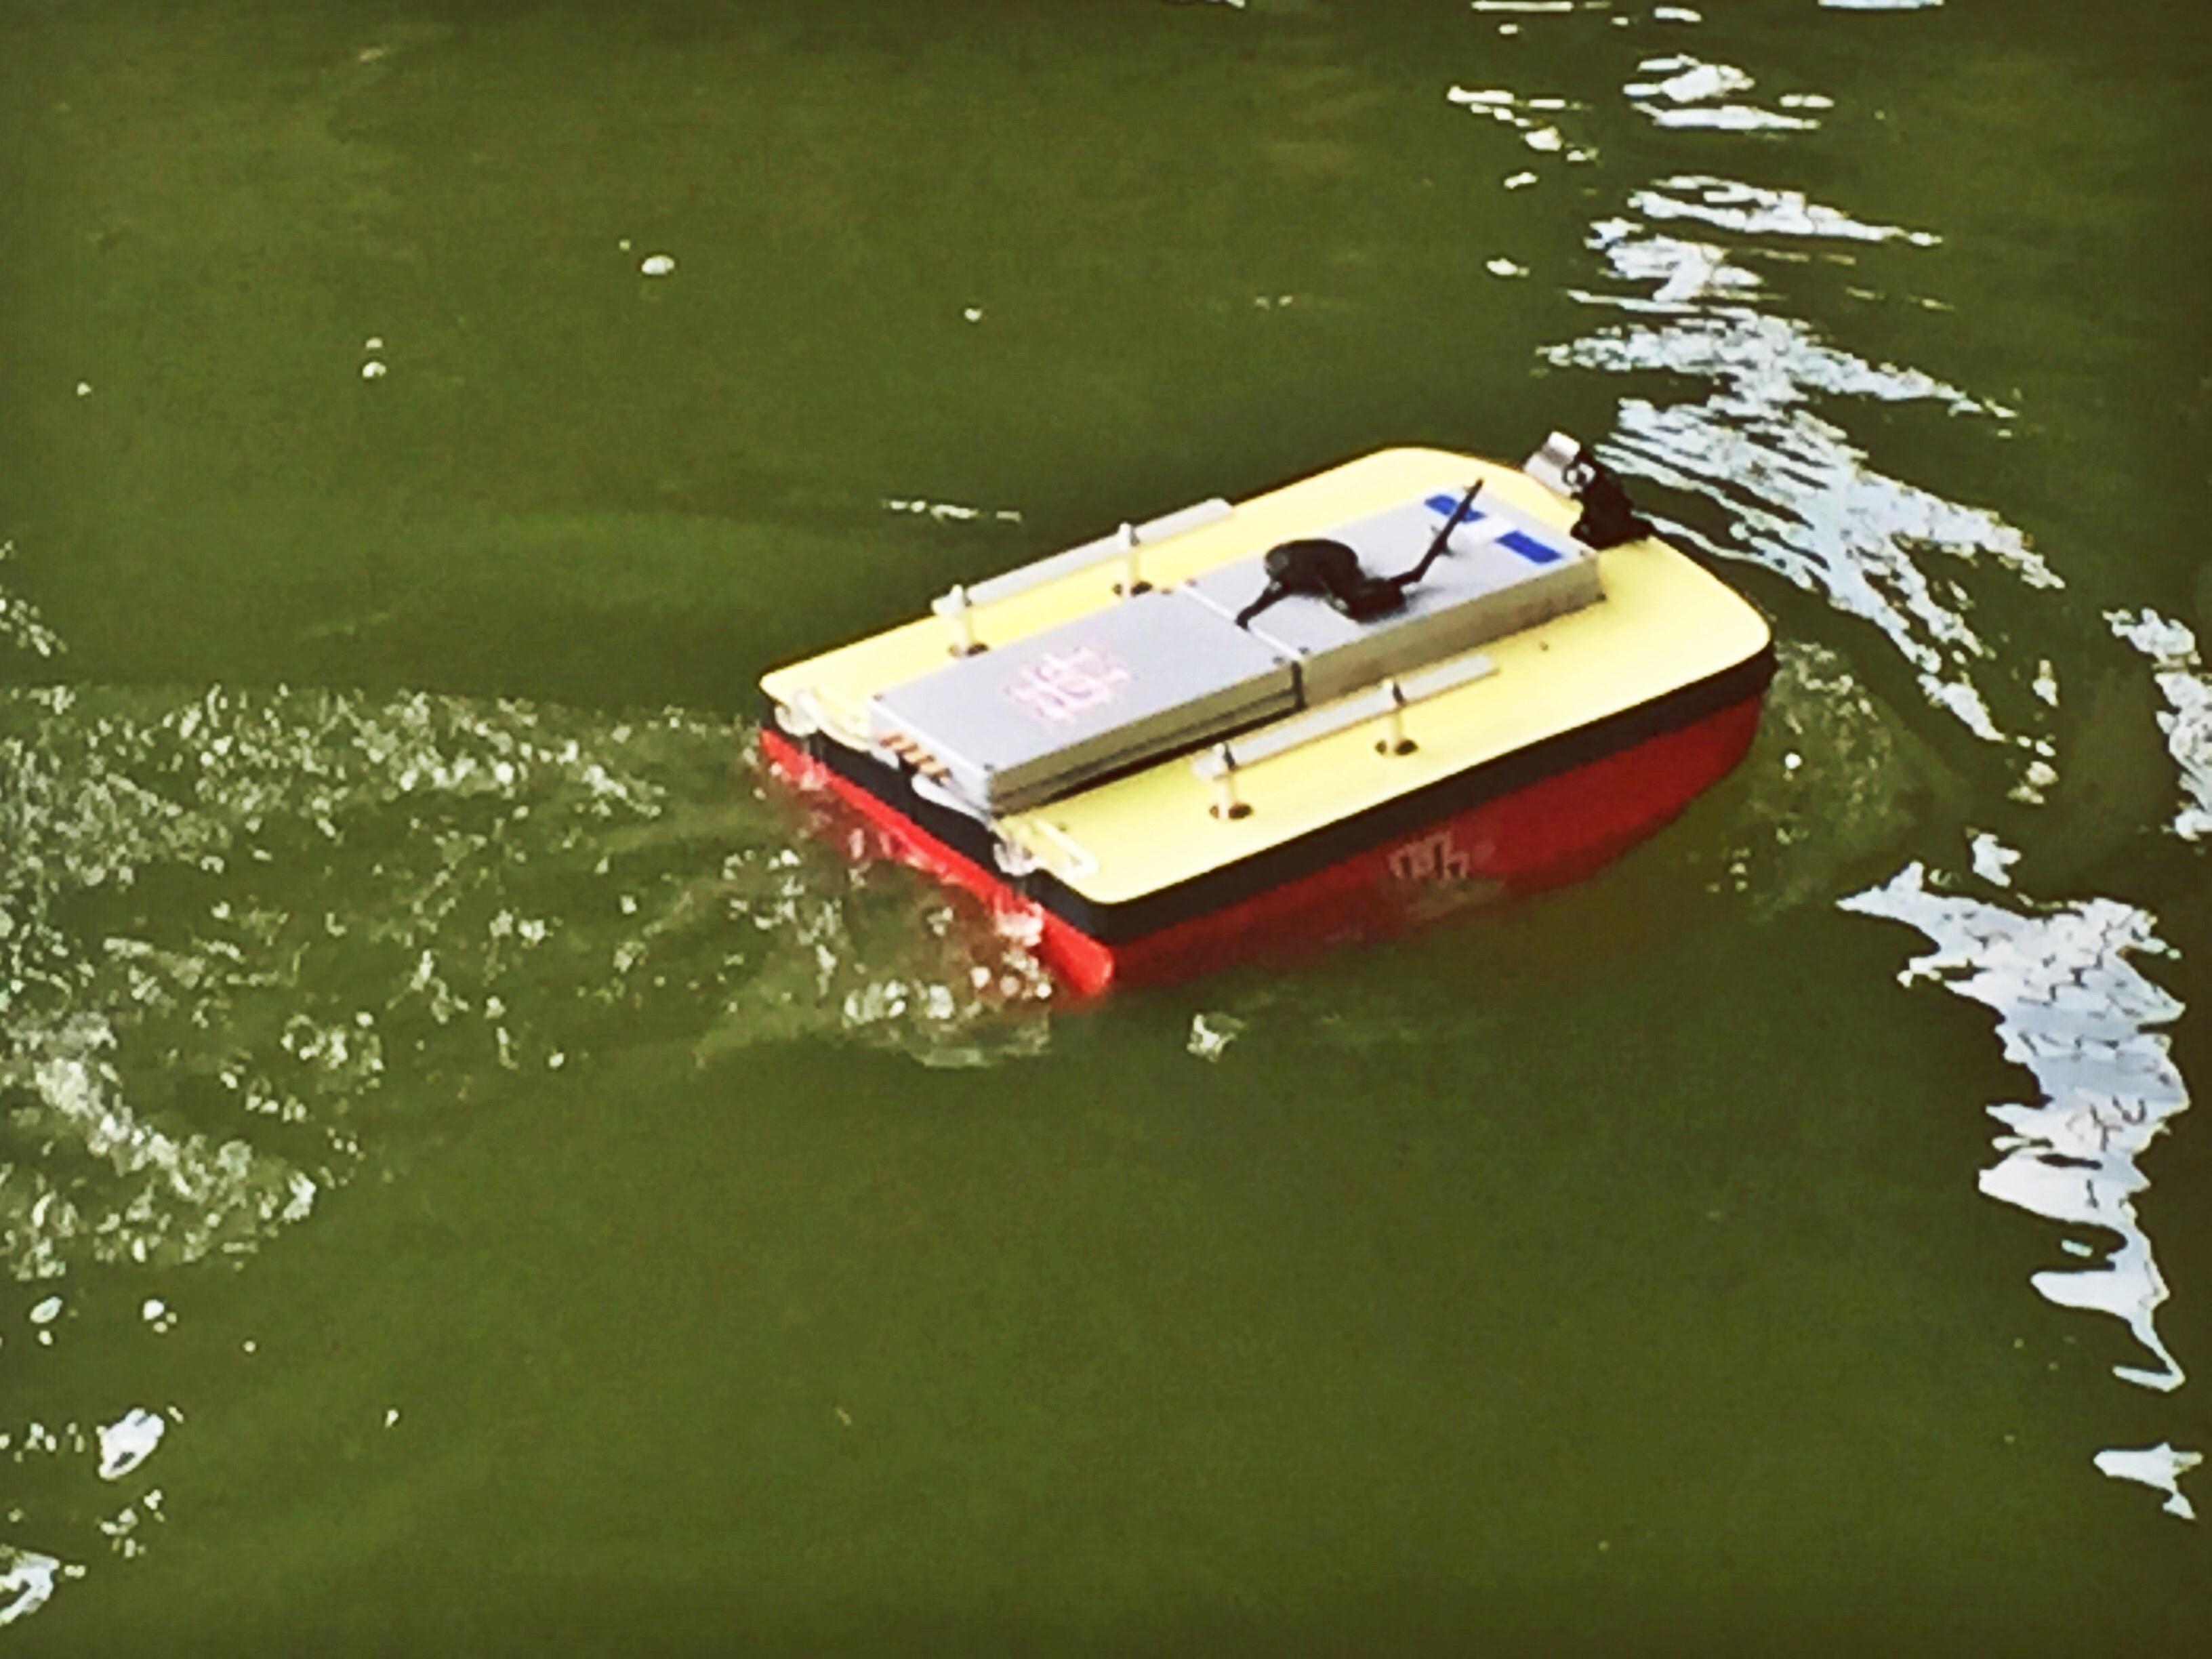
\includegraphics[width=.48\columnwidth]{driftnode/test1_1.jpg}
	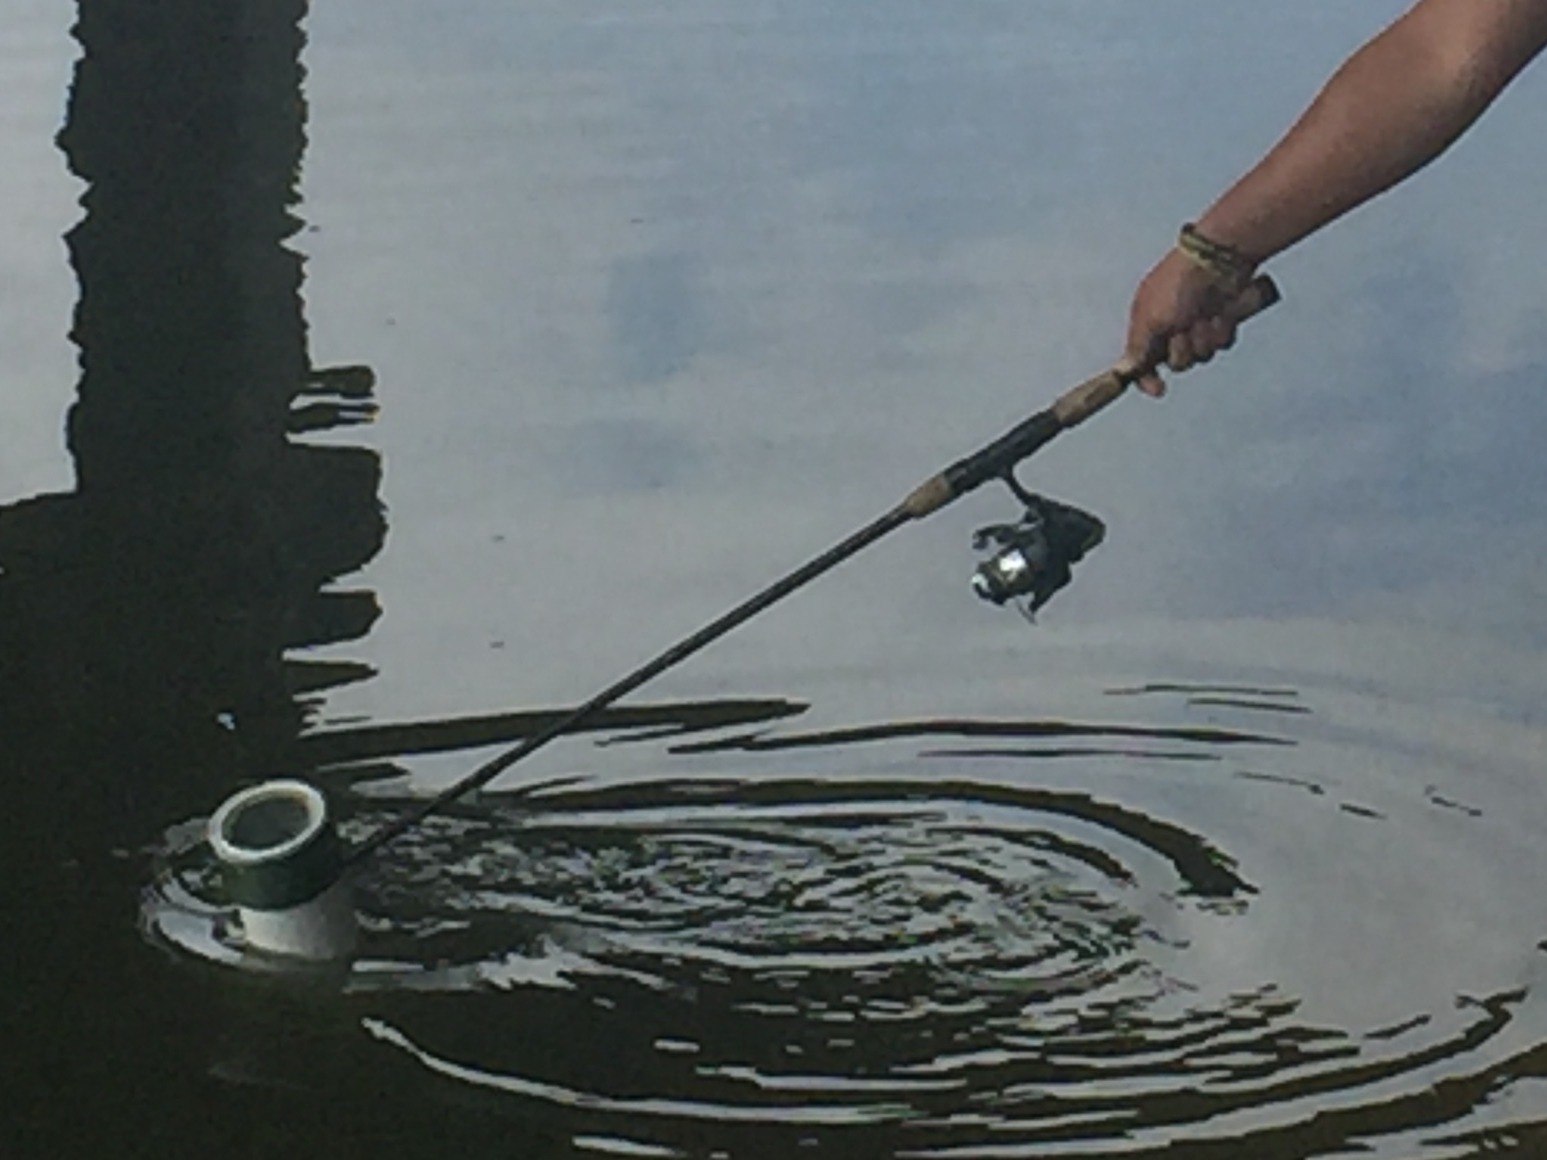
\includegraphics[width=.48\columnwidth]{driftnode/test1_2.jpg}
	\caption[MaxBotix first test]{
		Testing the driftnode by towing the waterproof assembly behind a remote controlled boat
	} \label{fig:boattest}
	\end{center}
	\vspace{-1em}
\end{figure}

Since we needed a mobile testing platform for our range sensors, a driftnode prototype was built that can accept different sensor caps.
The Maxbotix MB7380 was integrated to the driftnode's first prototype, to test its capabilities in real world condition.
As shown in Fig.~\ref{fig:boattest} we towed the driftnode assembly while it is logging data behind a remote controlled boat for the first test.
Our first test of the sensor showed that the sensor can differentiate between being submerged and in the air.
Fig.~\ref{fig:boattestlog} show the log file for the Maxbotix sensor, showing two distinct type of readings, where the lower, flatter reading is out of the water, and the higher, more variable reading is in the water.
However, the first test did not have another sensor that we know would work to measure depth, therefore we could not compare the Maxbotix sensor against a ground truth.

\begin{figure}[h]
	\begin{center}
	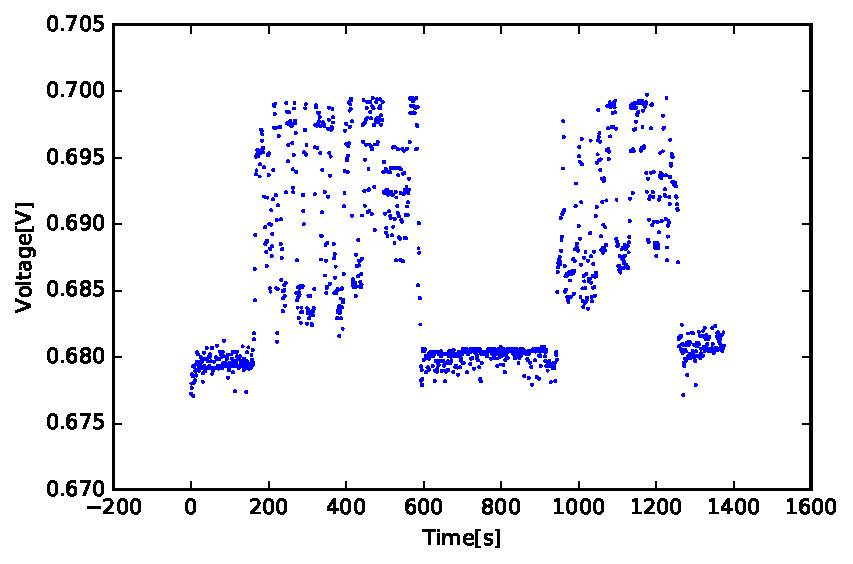
\includegraphics[width=.75\columnwidth]{driftnode/maxbotixlog1.pdf}
	\caption[MaxBotix first test]{
		Range sensor log of the first test
	} \label{fig:boattestlog}
	\end{center}
	\vspace{-1em}
\end{figure}

\begin{figure}[h]
	\begin{center}
	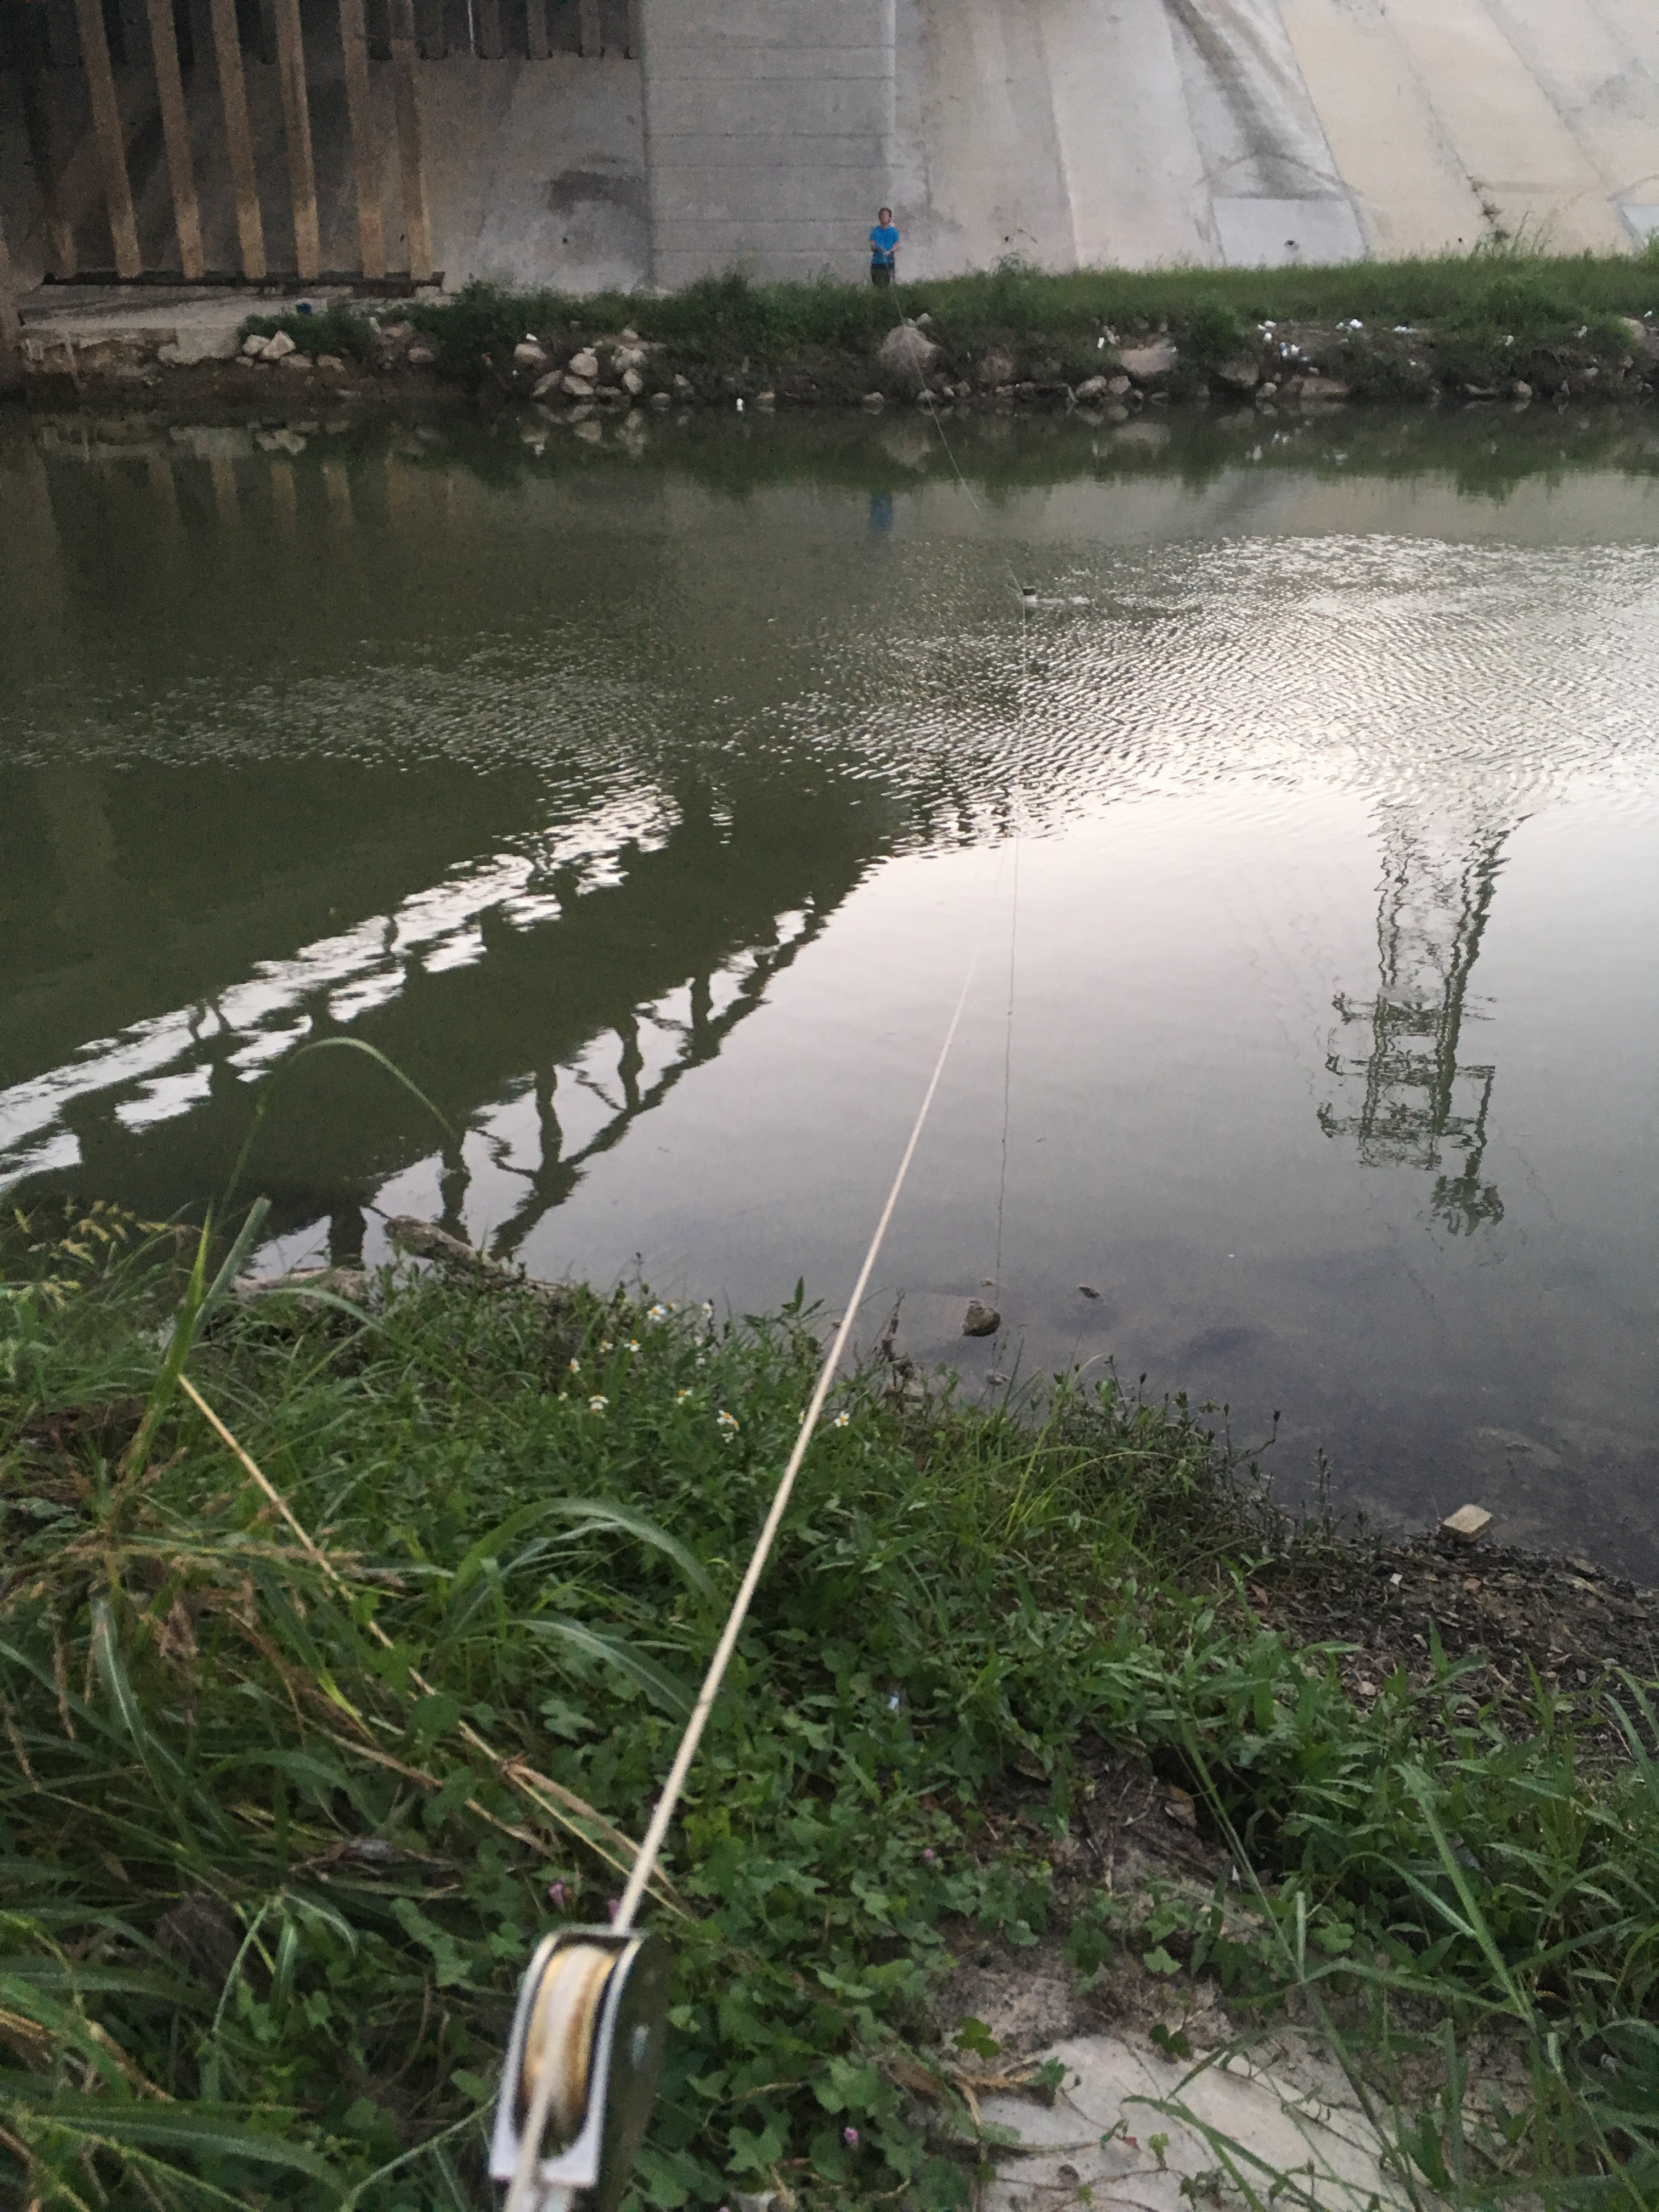
\includegraphics[height=6cm]{driftnode/pulleytest.jpg}
	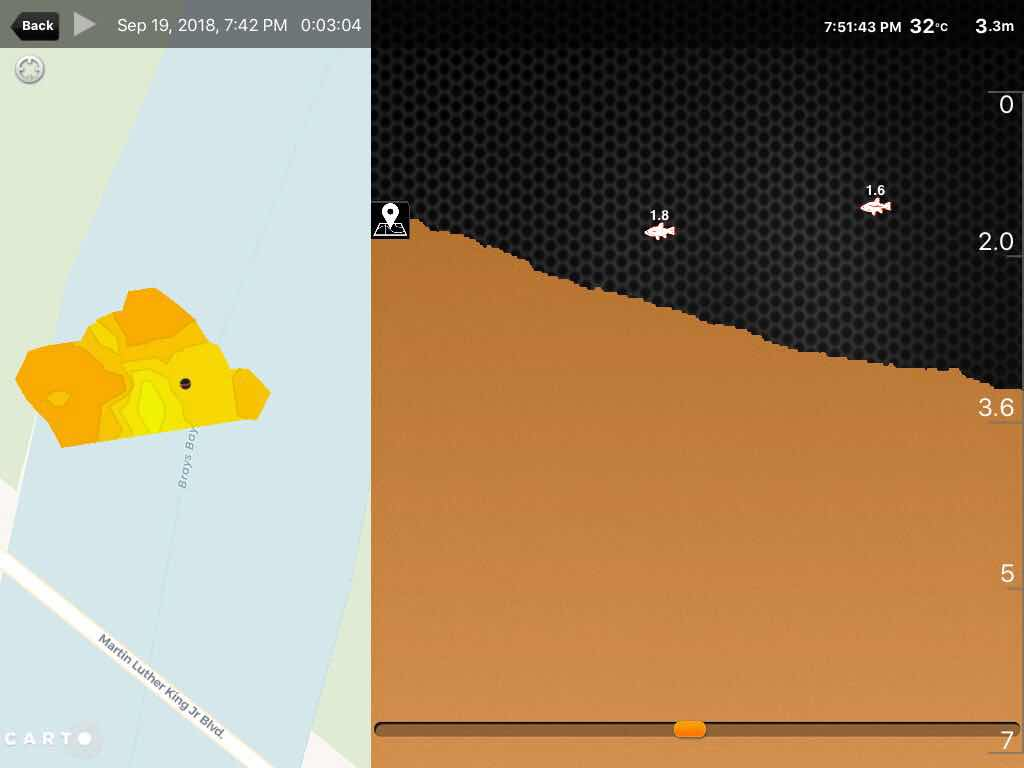
\includegraphics[height=6cm]{driftnode/fishfinderlog.jpg}
	\caption[Maxbotix pulley test]{
		(Left) testing set up for the second test of MaxBotix sensor
		(Right) output of the fish finder sensor
	} \label{fig:pulleytestsetup}
	\end{center}
	\vspace{-1em}
\end{figure}

The second test was to compare the sensor against a know ground truth.
We used a commercially available handheld wireless fishfinder, the Venterior VT-FF001 Portable Fish Finder, to compare against the MaxBotix sensor.
Ground anchors were established on each of the bayou's banks, opposite each other, where pulleys were attached and a string connecting the pulleys.
The sensors were pulled along the line for a repeatable path.
The fish finder data was used to compare against the MaxBotix sensor.
\begin{figure}[h]
	\begin{center}
	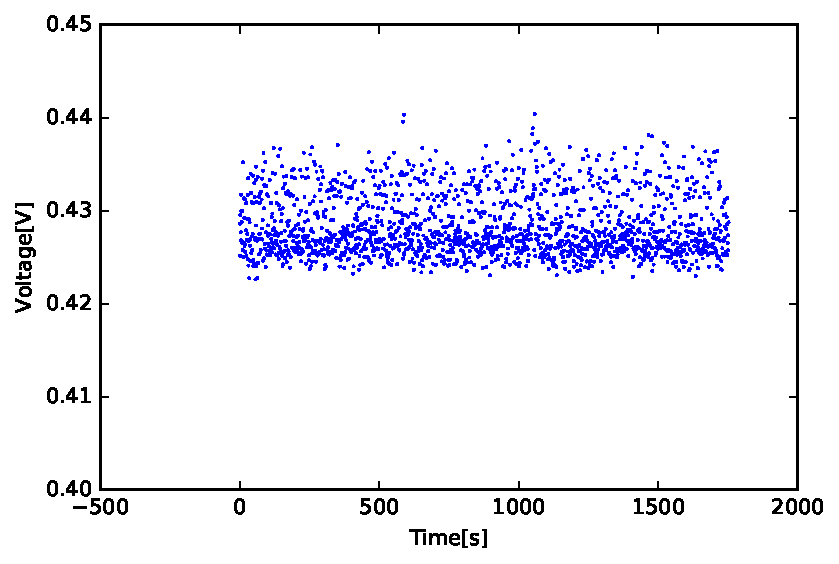
\includegraphics[width=.7\columnwidth]{driftnode/maxbotixlog2.pdf}
	\caption[Maxbotix pulley test log]{
		Maxbotix data log for the second test, noisy data that seems to be only noise
	} \label{fig:pulleylog}
	\end{center}
	\vspace{-1em}
\end{figure}

Fig.~\ref{fig:pulleytestsetup} show the second test's setup and a picture of the bottom of the bayou obtained with the fishfinder sensor.
Fig.~\ref{fig:pulleylog} show that the MaxBotix sensor returned data that was purely noise.
The second test showed that the MaxBotix is not usable as an underwater depth sensor.

\noindent  \emph{JSN-SR04T waterproof sensor}:

\begin{figure}[h]
	\begin{center}
	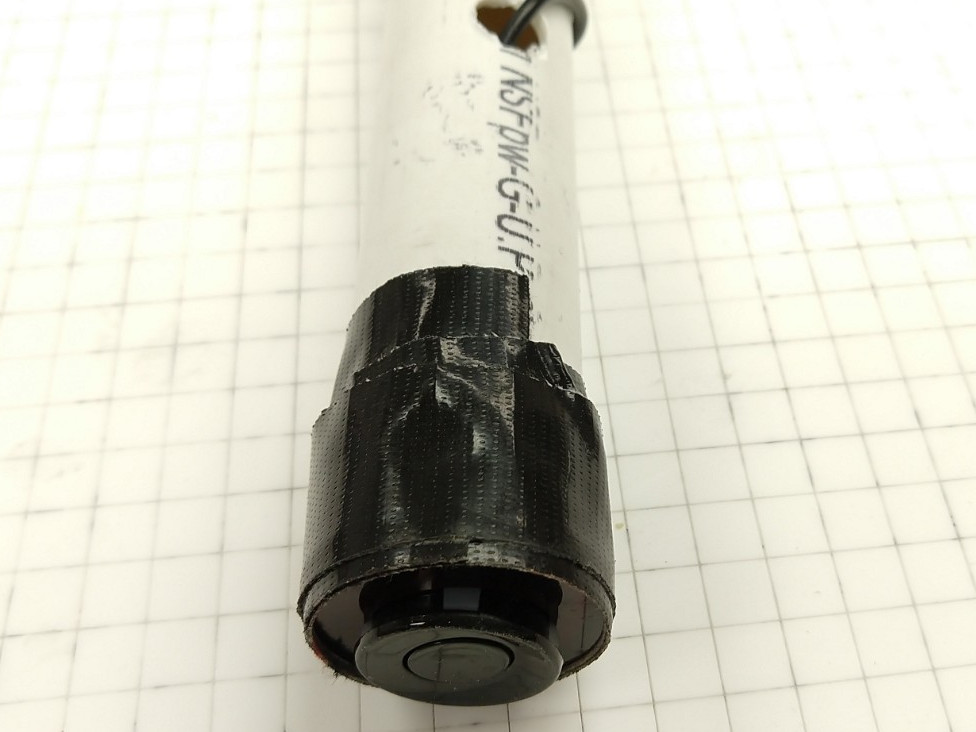
\includegraphics[width=.6\columnwidth]{driftnode/jsnsr04tpole.jpg}
	\caption[JSN-SR04T]{
		JSN-SR04T testing platform
	} \label{fig:jsnsr04t}
	\end{center}
	\vspace{-1em}
\end{figure}
The JSN-SR04T sensor seen in Fig.~\ref{fig:sonarsensors} is a basic, hobbyist level weatherized range sensor that have been shown to be capable of underwater depth sensing \cite{bakarsonar}. Fig.~\ref{fig:jsnsr04t} show the pole the sensor is attached to so that the sensor can be submerged at predetermined level.
\begin{figure}[h]
	\begin{center}
	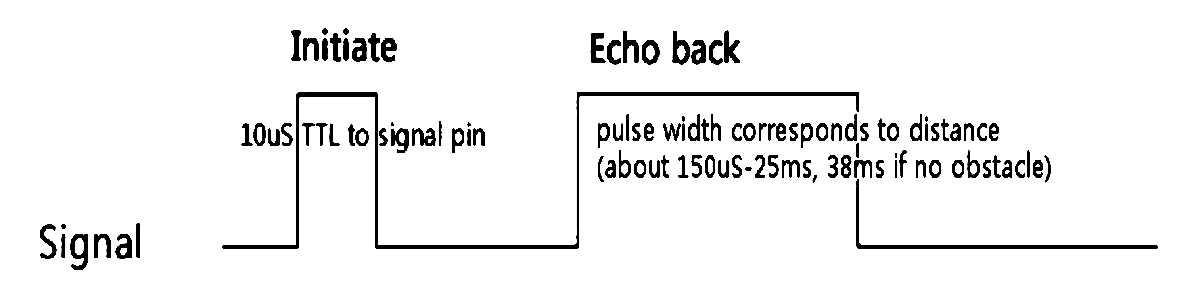
\includegraphics[width=.65\columnwidth]{driftnode/jsntiming.png}
	\caption[JSN-SR04T Timing]{
		Example signal of JSN-SR04T operation
	} \label{fig:jsntiming}
	\end{center}
	\vspace{-1em}
\end{figure}
The sensor timing diagram is shown in Fig.~\ref{fig:jsntiming}.
The sensor is attached to the end of a $\SI{1.15}{\metre}$ tall pole, which will allow the sensor to be submerged at a predetermined depth.
During testing, the pole was submerged into a $\SI{3.35}{\metre}$ deep pull, and every $\SI{15}{\second}$ the sensor was submerged $\SI{10}{\centi\metre}$ deeper.
Fig.~\ref{fig:jsnlog} show the log with of the sensor with respect to time.
A downward trend is clearly shown, with the maximum reading at $\SI{65}{\centi\metre}$, and minimum reading without noise is $\SI{40}{\centi\metre}$.
This correspond to an air distance of $\SI{2.84}{\metre}$ maximum and $\SI{1.7}{\metre}$ minimum.

\begin{figure}[h]
	\begin{center}
	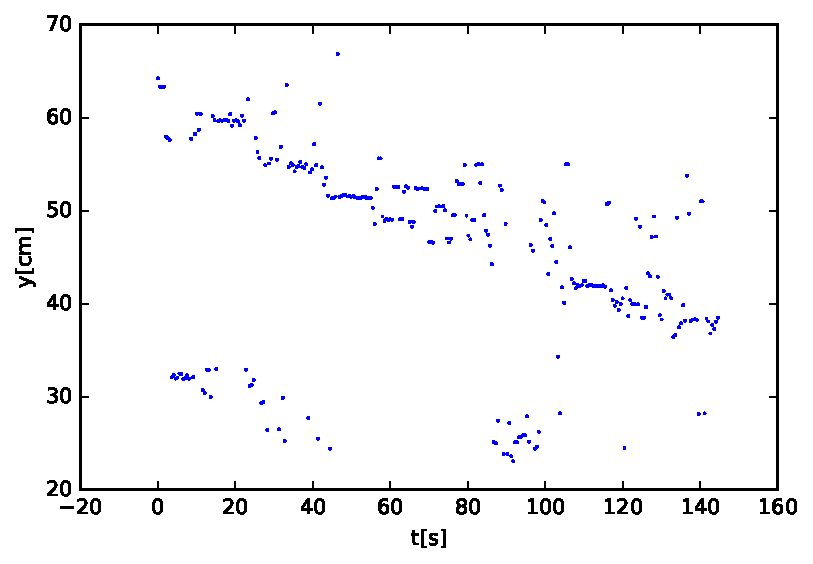
\includegraphics[width=.7\columnwidth]{driftnode/jsnlog.pdf}
	\caption[JSN-SR04T sensor log]{
		Log of the new sensor clear show a descending trend.
	} \label{fig:jsnlog}
	\end{center}
	\vspace{-1em}
\end{figure}
